\section{Numerical experiments}
In this section, we will firstly compare \texttt{expmber}, the new MATLAB implementation developed in this paper based on Bernoulli approximation, with the functions \texttt{exptaynsv3} \cite{RSID16}, that computes the matrix exponential using Taylor matrix polynomials, and \texttt{expm\_new} \cite{AlHi09} which implements a scaling squaring Pad\'e algorithm to work out the mentioned matrix function. 

Next, we will compare  \texttt{expmbertay}, the novel function that combines Taylor and Bernoulli approximations, with \texttt{expmber}, \texttt{exptaynsv3} and \texttt{expm\_new}. In \texttt{expmbertay}, the matrix exponential is carried out by means of Taylor series, when $m$ is less than or equal to 20, or Bernoulli series, when $m$ is equal to 25 or 30.

All the computations to obtain the {\it``exact"} matrix exponential function were carried out thanks to MATLAB's Symbolic Math Toolbox with 256 digit precision, using the \texttt{vpa} (variable-precision arithmetic) function.

\subsection{Experiments description}
The following test battery, composed of three types of different and representative matrices, has been chosen to compare the numerical performance of the above described codes:
\begin{itemize}
        \item[a)]  One hundred diagonalizable  $128 \times 128$ real matrices with 1-norms varying from 2.18 to 207.52. These matrices have the form  $A=VDV^T$, where
        $D$ is a diagonal matrix with real and complex eigenvalues and $V$ is an
        orthogonal matrix obtained as $V=H/\sqrt{128}$, being $H$ the Hadamard matrix.
        The {\it``exact"} matrix exponential was computed as $\exp(A)=V\exp(D)V^T$ (see \cite[pp. 10]{High08}).         

        \item[b)] One hundred non-diagonalizable $128 \times 128$ complex matrices with 1-norms ranging from 84 to 98. These matrices have the form $A=VJV^T$, where $J$ is a Jordan matrix with complex eigenvalues of modulus less than 10 and algebraic multiplicity random varying from 1 to 5. $V$ is an orthogonal matrix obtained as $V=H/\sqrt{128}$, where $H$ is the Hadamard matrix.
        The {\it``exact"} matrix exponential was worked out as $\exp(A)=V\exp(J)V^T$.         
        \item[c)] State-of-the-art matrices:\begin{itemize}
        \item Forty matrices from the Matrix Computation Toolbox (MCT) ~\cite{higham1995test}.
        \item Sixteen matrices from the Eigtool MATLAB package (EMP)~\cite{wrighteigtool} with sizes $127 \times 127$ and $128 \times 128$.
        
                         The {\it``exact"} matrix exponential for these matrices was computed by using Taylor approximations of orders 30, 36, 42, 49, 56 and 64, changing their scaling parameter (see Algorithm \ref{Alg_exp_exact}).         
        
                 Although the MCT and the EMP are initially composed of fifty-two and twenty matrices, respectively, twelve from the MCT and four from the EMP matrices were discarded for different reasons. For example, matrices 5, 10, 16, 17, 21, 25, 26, 42, 43, 44 and 49 belonging to the MCT and matrices 5 and 6 appertaining to the EMP were not taken into account since the exact exponential solution could not be computed. Besides, matrix 2 from the MCT and matrices 3 and 10 from the EMP were not considered because the excessively high relative error provided by all the methods to be compared.   
\end{itemize}         
       
\end{itemize}

\begin{algorithm}[H]
\caption{Computes the {\it``exact"} matrix exponential $B=e^{A}$,
where $A \in {\mathbb{C}^{r \times r}}$, by means of Taylor expansion using MATLAB function VPA with $n$ digits of precision.}
\label{Alg_exp_exact}
\begin{algorithmic} [1]
\State \textbf{If} there exits two consecutive orders $m_{k-1},m_{k}\in \left\{ {30,36,42,49,56,64} \right\}$ e integers $1 \le i,j \le 15$ such that
 \[\frac{{{{\left\| {B_{{m_{k - 1}}}^{(i)}(n) - B_{{m_{k - 1}}}^{(i - 1)}(n)} \right\|}_1}}}{{{{\left\| {B_{{m_{k - 1}}}^{(i)}(n)} \right\|}_1}}} < u\] and
\[\frac{{{{\left\| {B_{{m_k}}^{(j)}(n) - B_{{m_k}}^{(j - 1)}(n)} \right\|}_1}}}{{{{\left\| {B_{{m_k}}^{(j)}(n)} \right\|}_1}}} < u\]
and
\[\frac{{{{\left\| {B_{{m_k}}^{(j)}(n) - B_{{m_{k - 1}}}^{(i)}(n)} \right\|}_1}}}{{{{\left\| {B_{{m_k}}^{(j)}(n)} \right\|}_1}}} < u\]
by using Algorithm \ref{Alg_exp_vpa}

\textbf{Then}
\Return $B={B_{{m_k}}^{(j)}(n)}$

\textbf{Else}  \Return \textbf{Error} 
\end{algorithmic}
\end{algorithm}

\begin{algorithm}[H]
\caption{Computes $B^{(s)}_{m}(n)=e^{A}$,
where $A \in {\mathbb{C}^{r \times r}}$, by Taylor expansion of order $m$ and parameter scaling $s$ with $n$ digits of precession.}
\label{Alg_exp_vpa}
\begin{algorithmic} [1]

\State Compute $B^{(s)}_{m}(n) = {P_{m}}(A/2^{s})$ using Taylor
expansion of order $m$ with $n$ digits of precision
\For {$i=1:s$}
    \State $B^{(s)}_{m}(n)=[B^{(s)}_{m}(n)]^{2}$
 \EndFor
\end{algorithmic}
\end{algorithm}

For each of the sets of matrices described, an experiment, called Test, was respectively performed, evaluating the computational cost and the numerical accuracy of the methods under comparison. The three tests were executed using MATLAB (R2018b) running on an HP Pavilion dv8 Notebook PC with an Intel Core i7 CPU Q720 @1.60Ghz processor and 6 GB of RAM. 

\subsection{Experimental results}

Table \ref{table_prod_comparative} shows the computational costs of each method represented in terms of the number of matrix products (\texttt{P}), taking into account that the cost of the rest of the operations is negligible compared to it for big enough matrices. As can be seen, \texttt{expmber} and \texttt{exptaynsv3} achieved an identical number of matrix multiplications, since the same algorithm was used by both of them to calculate the degree of the polynomial ($m$) and the value of the scaling ($s$). This number of products was lower than that required by \texttt{expm\_new}, which gave rise to the highest computational cost. In addition to perform matrix products, \texttt{expm\_new} solves a system of linear equations with $n$ right-hand size vector where $n$ represents the size of the square coefficient matrix, whose computational cost was approximated as 4/3 matrix products.

%%%% Tables products
\begin{table}[!t]\begin{center}
        \caption{Matrix products (P) for  Tests 1, 2 and 3 using \texttt{expmber}, \texttt{exptaynsv3}
and \texttt{expm\_new} MATLAB codes.}
{\small
        \begin{tabular}{|c||c|c|c|}\hline&\texttt{P(expmber)}&\texttt{P(exptaynsv3)}&\texttt{P(expm\_new)}\\\hline
            Test 1 & 1131 & 1131 & 1178.33 \\\hline
            Test 2 & 1100 & 1100 & 1227.33 \\\hline
            Test 3 & 617  & 617  & 654.67 \\\hline
        \end{tabular}
}
        \label{table_prod_comparative}
    \end{center}
\end{table} 

Table \ref{table_err_comparative}, on the other hand, shows the percentage of cases in which the relative errors of \texttt{expmber} are lower, greater or equal than those of \texttt{exptaynsv3} and \texttt{expm\_new}. More in detail, the relative error was computed as
$$
\textmd{E}=\frac{\| \exp(A)-\tilde {exp}(A)\|_1}{\left\Vert
\exp(A)\right\Vert_1}
$$where $\tilde {exp}(A)$ is the approximate solution and $\exp(A)$ is the exact one.    

%%%% Tables error
% Table tests 
\begin{table}[!t]\begin{center}
                \caption{Relative error comparison among  \texttt{expmber}
vs  \texttt{exptaynsv3} and  \texttt{expmber}
vs  \texttt{expm\_new} for the three tests.}
{\small

               \begin{tabular}{|c||c|c|c|}\hline & Test 1  &Test 2 & Test 3\\\hline
                        E(\texttt{expmber})$<$E(\texttt{exptaynsv3})     & 56\% &  91\% & 30.36\%\\\hline
                        E(\texttt{expmber})$>$E(\texttt{exptaynsv3})     & 43\% &   9\%  & 62.5\%\\\hline
                        E(\texttt{expmber})$=$E(\texttt{exptaynsv3})     &  1\%  &   0\%  & 7.14\%\\\hline
                        E(\texttt{expmber})$<$E(\texttt{expm\_new})    & 97\% & 100\% & 69.64\%\\\hline
                        E(\texttt{expmber})$<$E(\texttt{expm\_new})    &   3\% &    0\% & 30.36\%\\\hline
                        E(\texttt{expmber})$=$E(\texttt{expm\_new})    &   0\% &    0\% &       0\%\\\hline
                \end{tabular}
}
                \label{table_err_comparative}
        \end{center}
\end{table}

With the exception of Test 3, the Bernoulli approach resulted in relative errors lower than those of Taylor one. With regard to Pad\'e, the Bernoulli algorithm always offered considerably more accurate results, which reached up to 100\% of the matrices for Test 2.

For the three tests, respectively, the normwise relative errors (a), the performance profiles (b), the ratio of the relative errors (c) and the ratio of the matrix products (d) among the distinct compared methods have been plotted in Figures ~\ref{fig:test1}, ~\ref{fig:test2}, and ~\ref{fig:test3}.

\begin{figure}[t]
\centering
\begin{subfigure}[b]{0.48\textwidth}
\includegraphics[scale=0.4]{Figures/normwise_exp_diag_hadamard_complex_n128_nd256_expmber.eps}
\caption{\footnotesize Normwise relative errors.} \label{fig:test1_a} \vspace{12pt}
\end{subfigure} \ \
\begin{subfigure}[b]{0.48\textwidth}
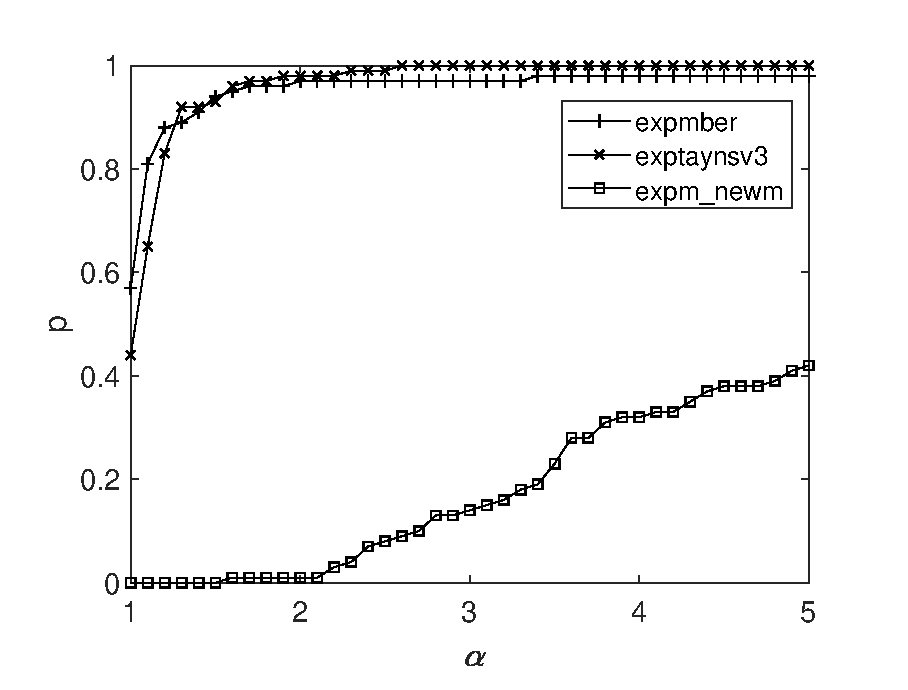
\includegraphics[scale=0.4]{Figures/nprofile_exp_diag_hadamard_complex_n128_nd256_expmber.eps}
\caption{\footnotesize Performance profile.}
\label{fig:test1_b}
\vspace{12pt}
\end{subfigure}
\begin{subfigure}[b]{0.48\textwidth}
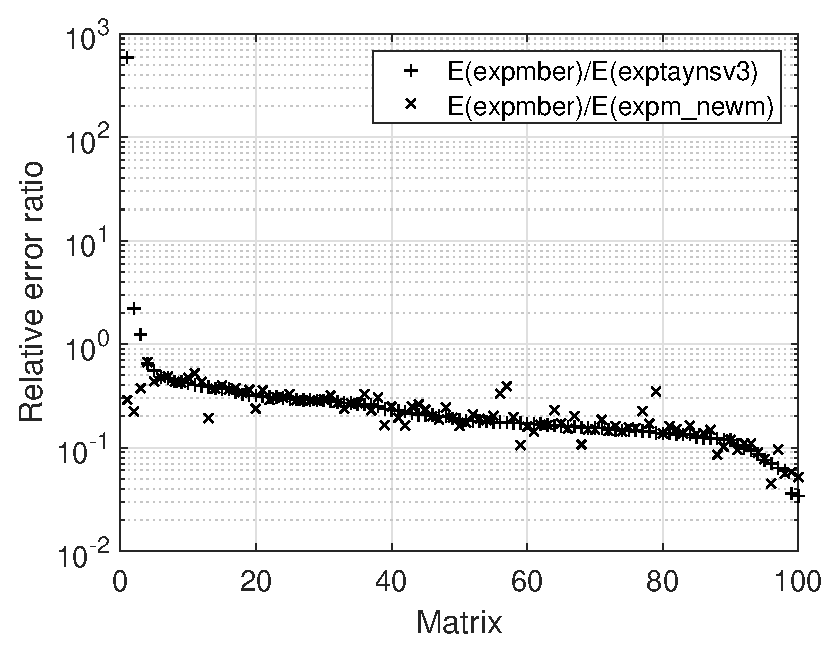
\includegraphics[scale=0.4]{Figures/error_ratio_exp_diag_hadamard_complex_n128_nd256_expmber.eps}
\caption{\footnotesize Ratio of relative errors.}
\label{fig:test1_c}
\end{subfigure}
\begin{subfigure}[b]{0.48\textwidth}
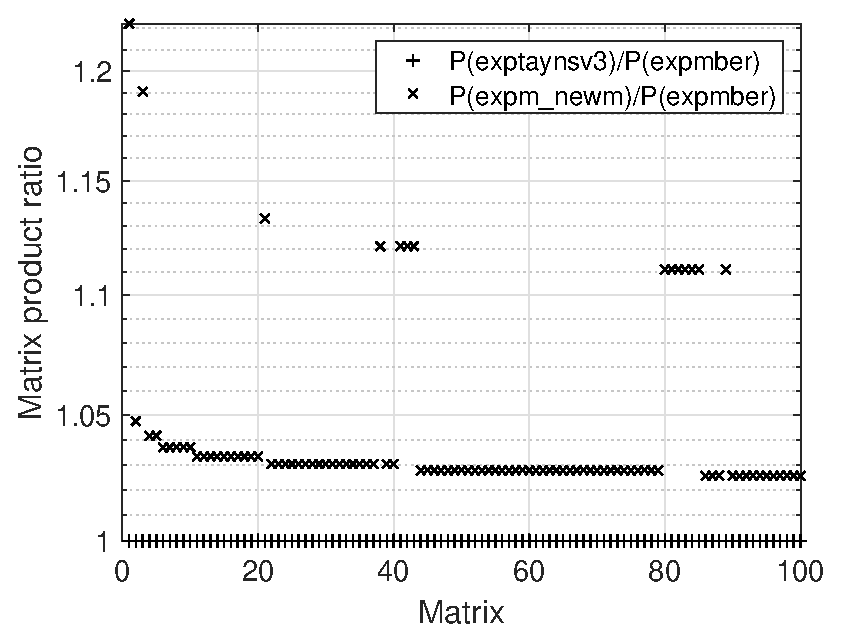
\includegraphics[scale=0.4]{Figures/matrix_product_ratio_exp_diag_hadamard_complex_n128_nd256_expmber.eps}
\caption{\footnotesize Ratio of matrix products.}
\label{fig:test1_d}
\end{subfigure}
\caption{Experimental results for Test~1.}
\label{fig:test1}
\end{figure}
        
\begin{figure}[t]
\centering
\begin{subfigure}[b]{0.48\textwidth}
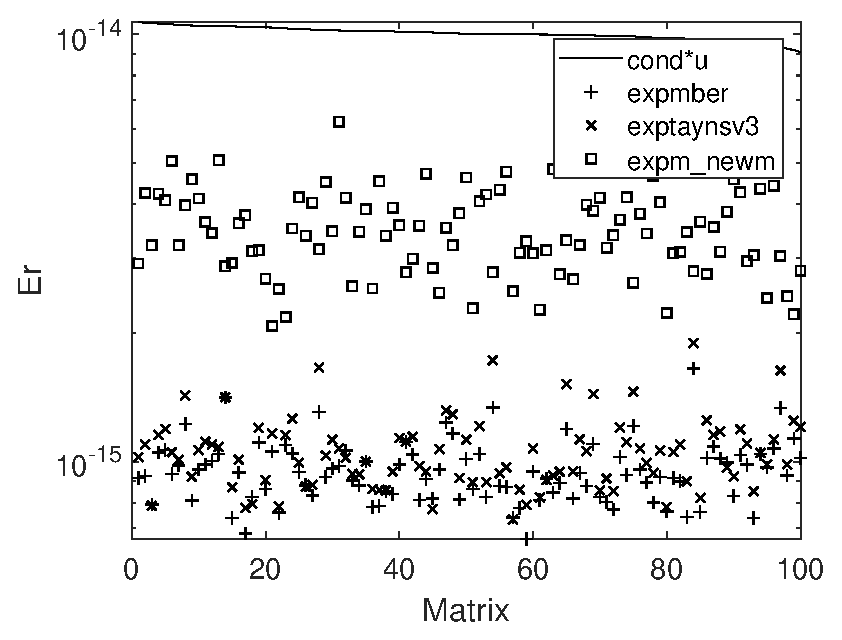
\includegraphics[scale=0.4]{Figures/normwise_exp_jordan_hadamard_complex_n128_boundvp10_maxmult5_nd256_expmber.eps}
\caption{\footnotesize Normwise relative errors.} \label{fig:test2_a} \vspace{12pt}
\end{subfigure} \ \
\begin{subfigure}[b]{0.48\textwidth}
\includegraphics[scale=0.4]{Figures/nprofile_exp_jordan_hadamard_complex_n128_boundvp10_maxmult5_nd256_expmber.eps}
\caption{\footnotesize Performance profile.}
\label{fig:test2_b}
\vspace{12pt}
\end{subfigure}
\begin{subfigure}[b]{0.48\textwidth}
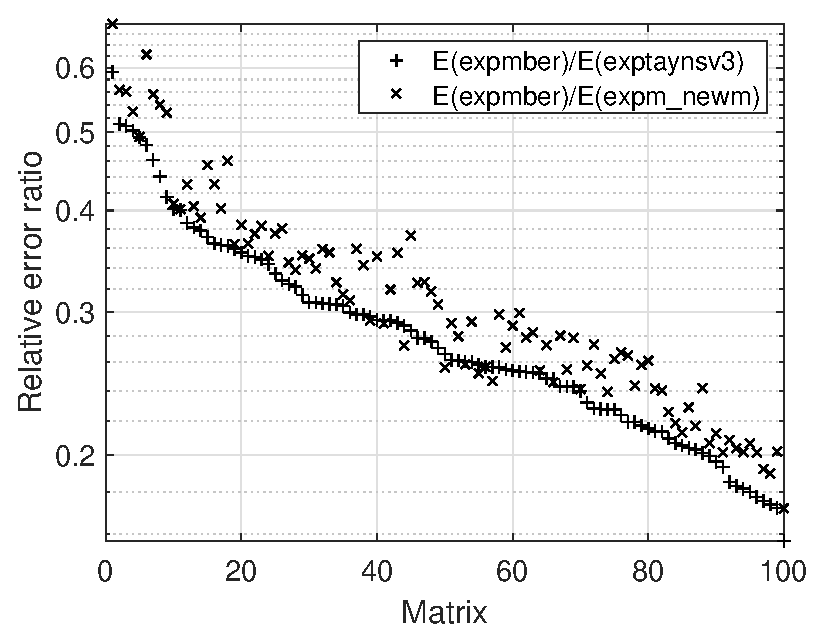
\includegraphics[scale=0.4]{Figures/error_ratio_exp_jordan_hadamard_complex_n128_boundvp10_maxmult5_nd256_expmber.eps}
\caption{\footnotesize Ratio of relative errors.}
\label{fig:test2_c}
\end{subfigure}
\begin{subfigure}[b]{0.48\textwidth}
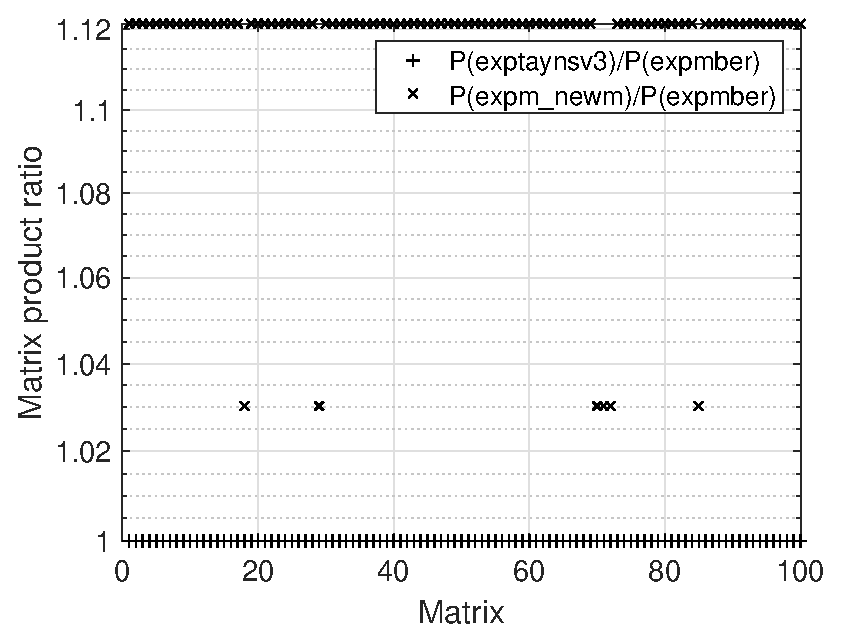
\includegraphics[scale=0.4]{Figures/matrix_product_ratio_exp_jordan_hadamard_complex_n128_boundvp10_maxmult5_nd256_expmber.eps}
\caption{\footnotesize Ratio of matrix products.}
\label{fig:test2_d}
\end{subfigure}
\caption{Experimental results for Test~2.}
\label{fig:test2}
\end{figure}

\begin{figure}[t]
\centering
\begin{subfigure}[b]{0.48\textwidth}
\includegraphics[scale=0.4]{Figures/normwise_exp_toolbox_n128_nd256-exp_eigtool_n128_nd256_expmber.eps}
\caption{\footnotesize Normwise relative errors.} \label{fig:test3_a} \vspace{12pt}
\end{subfigure} \ \
\begin{subfigure}[b]{0.48\textwidth}
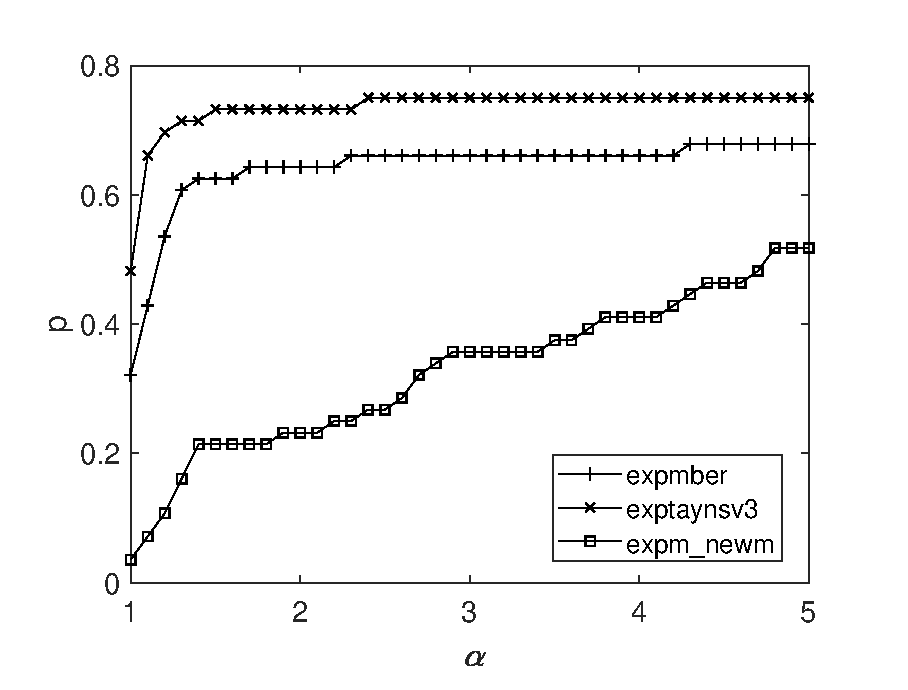
\includegraphics[scale=0.4]{Figures/nprofile_exp_toolbox_n128_nd256-exp_eigtool_n128_nd256_expmber.eps}
\caption{\footnotesize Performance profile.}
\label{fig:test3_b}
\vspace{12pt}
\end{subfigure}
\begin{subfigure}[b]{0.48\textwidth}
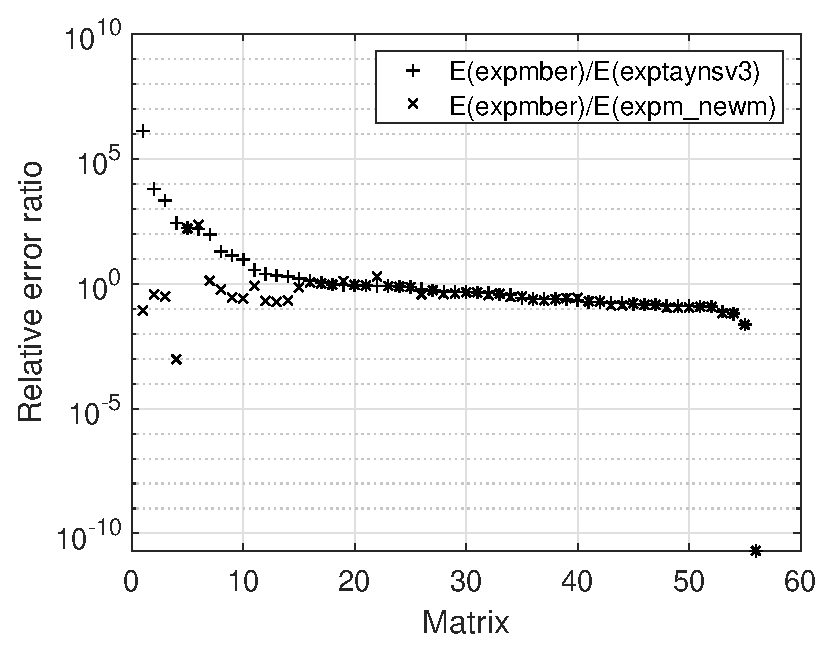
\includegraphics[scale=0.4]{Figures/error_ratio_exp_toolbox_n128_nd256-exp_eigtool_n128_nd256_expmber.eps}
\caption{\footnotesize Ratio of relative errors.}
\label{fig:test3_c}
\end{subfigure}
\begin{subfigure}[b]{0.48\textwidth}
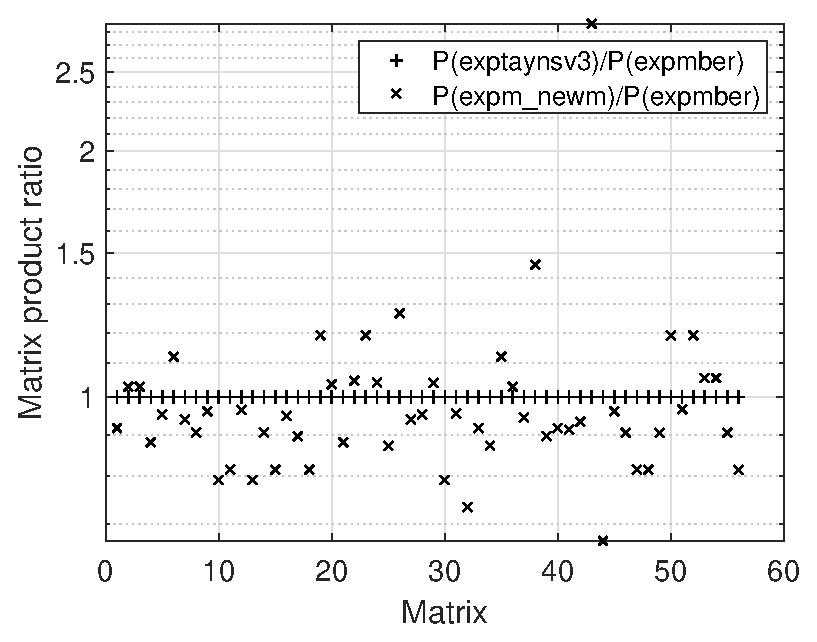
\includegraphics[scale=0.4]{Figures/matrix_product_ratio_exp_toolbox_n128_nd256-exp_eigtool_n128_nd256_expmber.eps}
\caption{\footnotesize Ratio of matrix products.}
\label{fig:test3_d}
\end{subfigure}
\caption{Experimental results for Test~3.}
\label{fig:test3}
\end{figure}

Regarding the normwise relative errors presented in Figures~\ref{fig:test1_a}, \ref{fig:test2_a} and \ref{fig:test3_a}, their solid line represents the function ${k_{\exp}}u$, where ${k_{\exp}}$ (or $cond$) is the condition number of the matrix exponential function \cite[Chapter 3]{High08} and $u=2^{-53}$ is the unit roundoff in the IEEE double precision floating-point arithmetic. \texttt{expmber} exhibited a very good numerical stability, in general. This can be appreciated seeing the distance from each matrix normwise relative error to the $cond*u$ line. In Figures~\ref{fig:test1_a} and \ref{fig:test2_a}, the numerical stability is even much better because these errors are below this line. Because ${k_{\exp}}$ was infinite or enormously high for the matrices 6, 7, 12, 15, 23, 36, 39, 50 and 51 from the MCT and for the matrices 1, 4, 8 and 15 from the EMP, all of them were rejected in the Figure \ref{fig:test3_a} visualisation but considered in the other ones.

In the performance profile Figures (\ref{fig:test1_b}, \ref{fig:test2_b} and \ref{fig:test3_b}), the $\alpha$ coordinate, on the $x$-axis, varies from 1 to 5 in steps equal to 0.1. For a concrete $\alpha$ value, the $p$ coordinate,  on the $y$-axis,  means the probability that the considered algorithm has a relative error lower than or equal to $\alpha$-times the smallest relative error over all the methods on the given test. For the first two tests (Figures~\ref{fig:test1_b}, \ref{fig:test2_b}), the performance profile shows that Bernoulli and Taylor method accuracy was similar. Both of them had much better correctness than the Pad\'e method. Nothwithstanding, Figure~\ref{fig:test3_b} reveals that \texttt{exptaynsv3} code improved the result accuracy against the \texttt{expmber} function, for the Test 3. 

In Figures \ref{fig:test1_c}, \ref{fig:test2_c} and \ref{fig:test3_c}, the ratios of relative errors have been presented in decreasing order with respect to E(\texttt{expmber})/E(\texttt{exptaynsv3}). They confirm the data exposed in Table \ref{table_err_comparative}, where it was shown that \texttt{expmber} provides a more accurate result than \texttt{exptaynsv3} for Tests 1 and 2, but not for Test 3. It is obvious to note that Pade offered worse performance in most cases.

In our opinion, this is clearly due to the distinctive numerical characteristics of the 3 sets of matrices analysed and the degree of the polynomial ($m$) required to be used. According to our experience, \texttt{expmber} provides results with a very appropriate accuracy for values of $m$ equal to 25 or 30. However, for significantly lower values, \texttt{expmber} will be less competitive than other codes, such as \texttt{exptaynsv3}. Minimum, maximum and average values of $m$ required for Tests 1, 2 and 3 are collected in Table \ref{table_m_comparative}. In more detail, Figure \ref{fig:m_value} shows the approximation polynomial order employed in the calculation of the exponential function by means of \texttt{expmber} (or \texttt{exptaynsv3}) and \texttt{expm\_new} for each of the matrices that are part of the test battery.

%%%% Table degree of polynomial
\begin{table}[!t]\begin{center}
        \caption{Mininum, maximum and average polynomial degree (m) required for Tests 1, 2 and 3 using \texttt{expmber} or \texttt{exptaynsv3} functions.}
{\small
        \begin{tabular}{|c||c|c|c|}\hline & Minimum & Maximum & Average \\\hline
            Test 1 & 16 & 30 & 27.51 \\\hline
            Test 2 & 30 & 30 & 30 \\\hline
            Test 3 & 12 & 30 & 25.70 \\\hline
        \end{tabular}}
        \label{table_m_comparative}
    \end{center}
\end{table} 


\begin{figure}[t]
\centering
\begin{subfigure}[b]{0.48\textwidth}
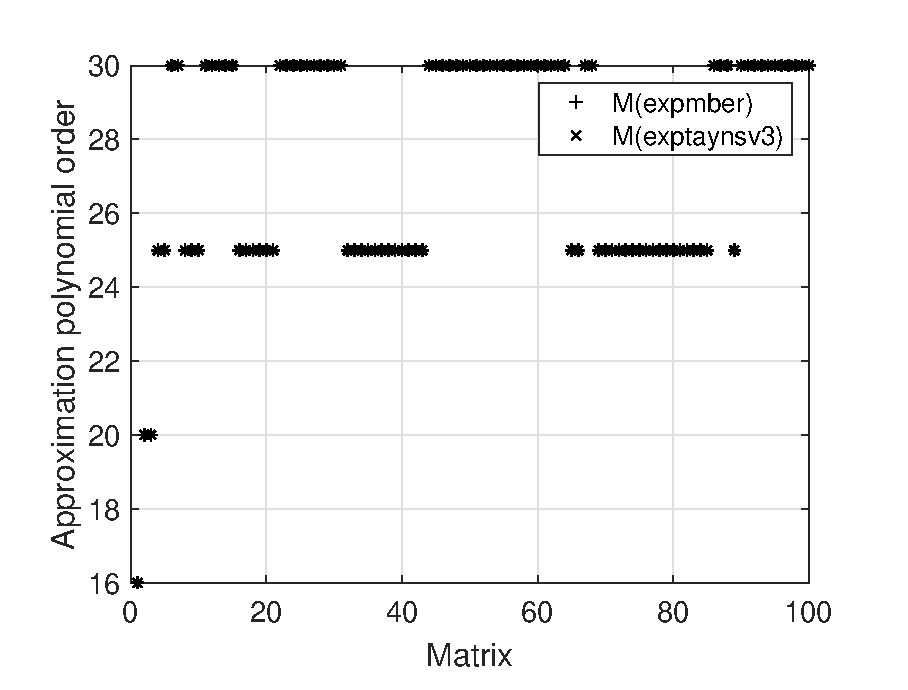
\includegraphics[scale=0.4]{Figures/polynomial_order_exp_diag_hadamard_complex_n128_nd256_expmber.eps}
\caption{\footnotesize Test~1.} \label{fig:m_value_test1} \vspace{12pt}
\end{subfigure} \ \
\begin{subfigure}[b]{0.48\textwidth}
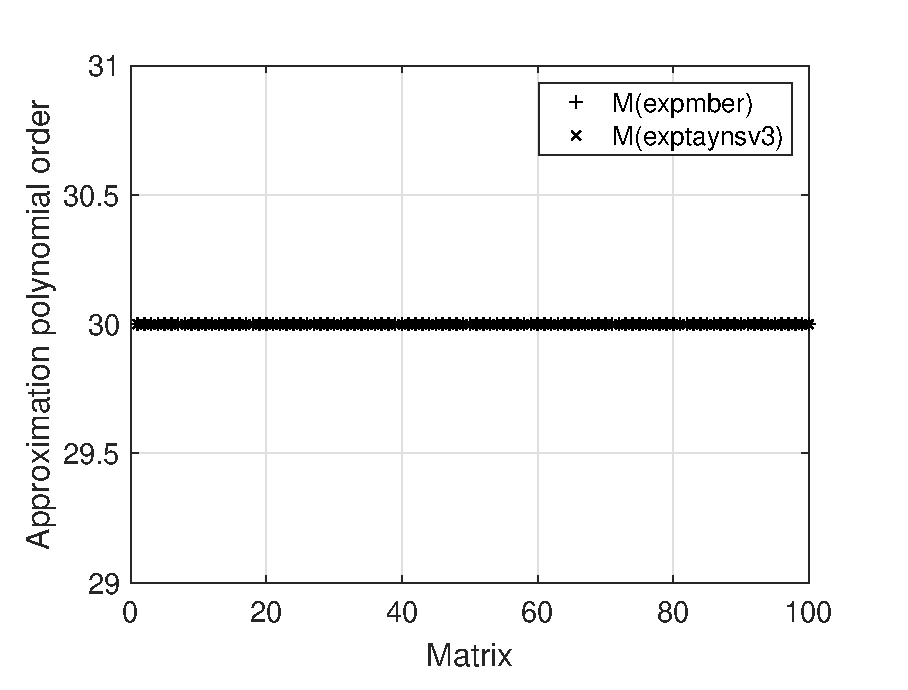
\includegraphics[scale=0.4]{Figures/polynomial_order_exp_jordan_hadamard_complex_n128_boundvp10_maxmult5_nd256_expmber.eps}
\caption{\footnotesize Test~2.}
\label{fig:m_value_test2}
\vspace{12pt}
\end{subfigure}
\begin{subfigure}[b]{0.48\textwidth}
\includegraphics[scale=0.4]{Figures/polynomial_order_exp_toolbox_n128_nd256-exp_eigtool_n128_nd256_expmber.eps}
\caption{\footnotesize Test~3.}
\label{fig:m_value_test3}
\end{subfigure}
\caption{Polynomial order (m) for Test~1, 2 and 3.}
\label{fig:m_value}
\end{figure}

As it was presented in Table \ref{table_prod_comparative}, \texttt{expmber} and \texttt{exptaynsv3} functions performed a lower number of matrix operations than \texttt{expm\_new} one. This statement can be also corroborated from the results displayed in Figures \ref{fig:test1_d}, \ref{fig:test2_d} and \ref{fig:test3_d}, where the ratio between the number of \texttt{expm\_new} and \texttt{expmber} matrix products ranged from 1.03 to 1.22 for Test 1, from 1.03 to 1.12 for Test 2 and from 0.67 to 2.87 for Test 3.

Next, we will analyse the possibility of using Bernoulli and Taylor methods together, giving place to a novel approach to compute the matrix exponential function. For that, we will start getting the benefits of the \texttt{exptaynsv3} function against \texttt{expm\_new} one.  As Table \ref{table_err_comparative_exptaynsv3} shows, the percentage of cases in which Taylor relative error is lower than Pad\'e reaches 100\% for Test 1 and 89.29\% for Test 3. Evidently, these error percentages improve those offered by Bernoulli approximation. 

%%%% Tables error
% Table tests 
\begin{table}[!t]\begin{center}
                \caption{Relative error comparison between \texttt{exptaynsv3} and \texttt{expm\_new} for the three tests.}
{\small
               \begin{tabular}{|c||c|c|c|}\hline & Test 1  &Test 2 & Test 3\\\hline
                        E(\texttt{exptaynsv3})$<$E(\texttt{expm\_new})    & 100\% & 100\% & 89.24\%\\\hline
                        E(\texttt{exptaynsv3})$>$E(\texttt{expm\_new})    &   3\% &     0\%  & 10.71\%\\\hline
                        E(\texttt{exptaynsv3})$=$E(\texttt{expm\_new})    &   0\% &     0\%  &       0\%\\\hline
                \end{tabular}}
                \label{table_err_comparative_exptaynsv3}
        \end{center}
\end{table}

From these excellent results, we therefore considered the possibility of combining Bernoulli and Taylor methods, giving rise to the \texttt{expmbertay} code. In this function, and as previously mentioned, we will use the Taylor approach (\texttt{exptaynsv3}) for values of m below 25 and the Bernoulli approximation ( \texttt{expmber}) when m equals 25 or 30. In this way, the number of matrix products needed by \texttt{expmbertay} will obviously be identical to that of \texttt{expmber} or \texttt{exptaynsv3}. 

Table \ref{table_err_comparative_expmbertay} collects thus the percentage of matrices in which the relative errors of \texttt{expmbertay} are lower, greater or equal than those of \texttt{exptaynsv3}, \texttt{expmber}  and \texttt{expm\_new}.  For the vast majority of matrices, \texttt{expmbertay} provided an accuracy in the results identical to that of \texttt{expmber}, improving even the latter by 23.21\% for the matrices of Test 3. With respect to \texttt{exptaynsv3}, \texttt{expmbertay} also enhanced the results achieved by \texttt{expmber}, so that this combined method is now better or equal than \texttt{exptaynsv3} in 55.36 percent of cases for Test 3. Moreover, \texttt{expmbertay} became better than \texttt{expm\_new} in 100\% of the matrices for Test 1 and 2, and 91.07\% for Test 3, which is higher than the percentages individually offered by \texttt{expmber} (69.64\%) and \texttt{exptaynsv3} (89.29\%).

%%%% Tables error
% Table tests 
\begin{table}[!t]\begin{center}
                \caption{Relative error comparison among \texttt{expmbertay} vs \texttt{exptaynsv3}, \texttt{expmbertay} vs \texttt{expmber}, and \texttt{expmbertay} vs \texttt{expm\_new} for the three tests.}
{\small
               \begin{tabular}{|c||c|c|c|}\hline & Test 1  &Test 2 & Test 3\\\hline
                        E(\texttt{expmbertay})$<$E(\texttt{exptaynsv3})    &   57\%  &   91\%  & 44.64\%\\\hline
                        E(\texttt{expmbertay})$>$E(\texttt{exptaynsv3})    &   42\%  &     9\%  & 44.64\%\\\hline
                        E(\texttt{expmbertay})$=$E(\texttt{exptaynsv3})    &     1\%  &     0\% &  10.72\%\\\hline
                        E(\texttt{expmbertay})$<$E(\texttt{expmber})       &     3\%  &     0\%  & 23.21\%\\\hline
                        E(\texttt{expmbertay})$>$E(\texttt{expmber})       &     0\%  &     0\%  &    0\%\\\hline
                        E(\texttt{expmbertay})$=$E(\texttt{expmber})       &   97\%  &  100\%  & 76.79\%\\\hline
                        E(\texttt{expmbertay})$<$E(\texttt{expm\_new})   & 100\%  & 100\%  &  91.07\%\\\hline
                        E(\texttt{expmbertay})$>$E(\texttt{expm\_new})   &    0\%  &     0\%  &  8.93\%\\\hline
                        E(\texttt{expmbertay})$<$E(\texttt{expm\_new})   &    0\%  &     0\%  &       0\%\\\hline
                \end{tabular}}
                \label{table_err_comparative_expmbertay}
        \end{center}
\end{table}

Numerical features of \texttt{expmbertay} are finally exposes in Figures \ref{fig:test4}, \ref{fig:test5} and \ref{fig:test6} for the three tests by means of the normwise relative errors (a), the performance profiles (b) and the ratio of the relative errors (c). As it can be seen, the method presents an excellent precision in the results, with very low relative errors, a very high probability in the performance profile pictures and .
\begin{figure}[t]
\centering
\begin{subfigure}[b]{0.48\textwidth}
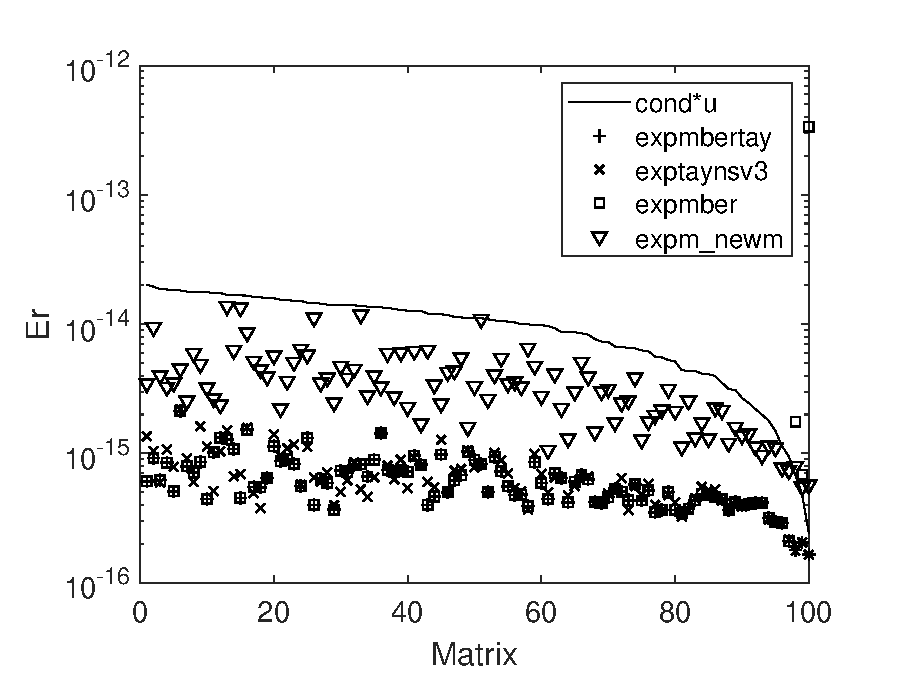
\includegraphics[scale=0.4]{Figures/normwise_exp_diag_hadamard_complex_n128_nd256_expmbertay.eps}
\caption{\footnotesize Normwise relative errors.} \label{fig:test4_a} \vspace{12pt}
\end{subfigure} \ \
\begin{subfigure}[b]{0.48\textwidth}
\includegraphics[scale=0.4]{Figures/nprofile_exp_diag_hadamard_complex_n128_nd256_expmbertay.eps}
\caption{\footnotesize Performance profile.}
\label{fig:test4_b}
\vspace{12pt}
\end{subfigure}
\begin{subfigure}[b]{0.48\textwidth}
\includegraphics[scale=0.4]{Figures/error_ratio_exp_diag_hadamard_complex_n128_nd256_expmbertay.eps}
\caption{\footnotesize Ratio of relative errors.}
\label{fig:test4_c}
\end{subfigure}
\caption{Experimental results for Test~1.}
\label{fig:test4}
\end{figure}
        
\begin{figure}[t]
\centering
\begin{subfigure}[b]{0.48\textwidth}
\includegraphics[scale=0.4]{Figures/normwise_exp_jordan_hadamard_complex_n128_boundvp10_maxmult5_nd256_expmbertay.eps}
\caption{\footnotesize Normwise relative errors.} \label{fig:test5_a} \vspace{12pt}
\end{subfigure} \ \
\begin{subfigure}[b]{0.48\textwidth}
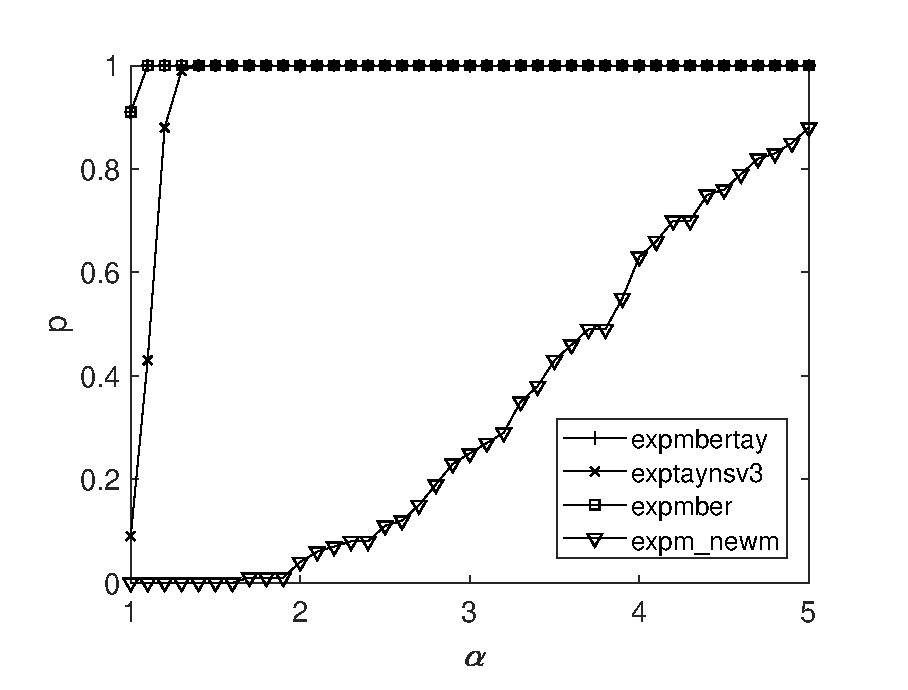
\includegraphics[scale=0.4]{Figures/nprofile_exp_jordan_hadamard_complex_n128_boundvp10_maxmult5_nd256_expmbertay.eps}
\caption{\footnotesize Performance profile.}
\label{fig:test5_b}
\vspace{12pt}
\end{subfigure}
\begin{subfigure}[b]{0.48\textwidth}
\includegraphics[scale=0.4]{Figures/error_ratio_exp_jordan_hadamard_complex_n128_boundvp10_maxmult5_nd256_expmbertay.eps}
\caption{\footnotesize Ratio of relative errors.}
\label{fig:test5_c}
\end{subfigure}
\caption{Experimental results for Test~2.}
\label{fig:test5}
\end{figure}

\begin{figure}[t]
\centering
\begin{subfigure}[b]{0.48\textwidth}
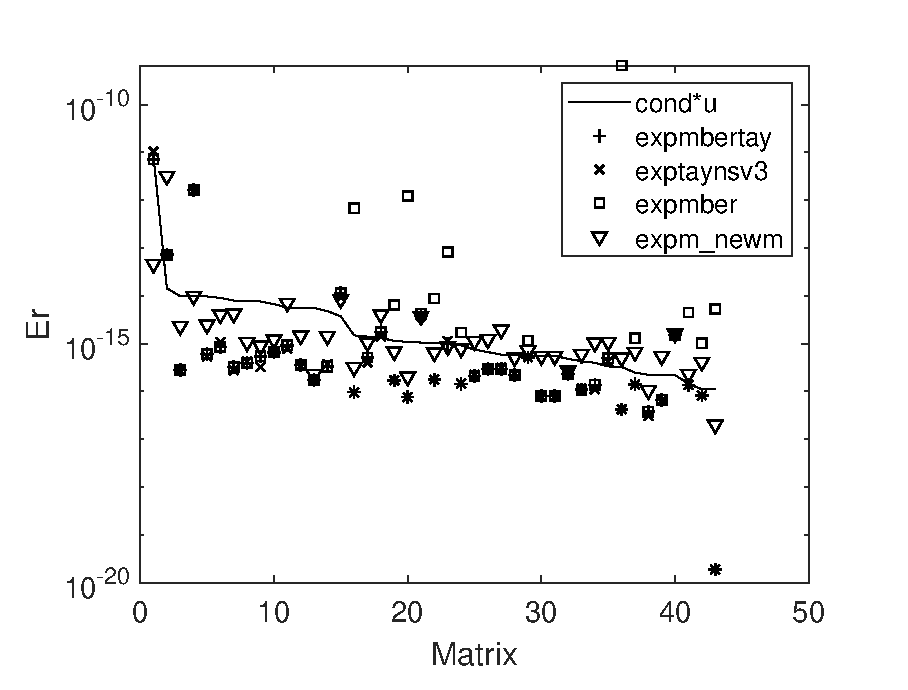
\includegraphics[scale=0.4]{Figures/normwise_exp_toolbox_n128_nd256-exp_eigtool_n128_nd256_expmbertay.eps}
\caption{\footnotesize Normwise relative errors.} \label{fig:test6_a} \vspace{12pt}
\end{subfigure} \ \
\begin{subfigure}[b]{0.48\textwidth}
\includegraphics[scale=0.4]{Figures/nprofile_exp_toolbox_n128_nd256-exp_eigtool_n128_nd256_expmbertay.eps}
\caption{\footnotesize Performance profile.}
\label{fig:test6_b}
\vspace{12pt}
\end{subfigure}
\begin{subfigure}[b]{0.48\textwidth}
\includegraphics[scale=0.4]{Figures/error_ratio_exp_toolbox_n128_nd256-exp_eigtool_n128_nd256_expmbertay.eps}
\caption{\footnotesize Ratio of relative errors.}
\label{fig:test6_c}
\end{subfigure}
\caption{Experimental results for Test~3.}
\label{fig:test6}
\end{figure}


%\section{Parallel algorithm}
\subsection{Results in GPU}

%As we did in~\cite{cosineHermite2019} 
We have implemented an ``accelerated'' version that allows to execute our algorithm
to compute the hyperbolic cosine on \nvidia\  GPUs.
Current GPUs are computational devices that allow to boost performance on data parallelism applications, i.e. applications that operate over many independent data.
This is the case of matrix multiplication, which is a highly optimized operation for GPUs in its current implementation routine included in the CUBLAS~\cite{CuLi09} package.
%Since our GPU algorithms are all based on Taylor approximations, which are rich in matrix products, we can get the best out of these devices.
Our GPU algorithms are all based on polynomial evaluations which, in turn, results in intensive use of matrix products. 
Matrix multiplication is a very optimized operation for GPU.

We have carried out our experimental results on a computer equipped with two processors Intel Xeon CPU E5-2697 v2 @2.70GHz featuring 12 cores each.
To obtain the algorithm performance on GPU we used one \nvidia Tesla K20Xm (Kepler architecture) attached to the PCI of this workstation.
This GPU features 2688 CUDA cores and 16 GB of memory.

\begin{figure}[!t]
        \setlength{\tabcolsep}{-10pt}
        \begin{center}
                %\begin{tabular}{cc}
                %\hspace{12pt}
                %\includegraphics[width=0.80\textwidth]{Tiempoparalelo.eps}
                \includegraphics[scale=0.9]{Figures/Tiempoparalelo.eps}
                %\includegraphics[width=0.57\textwidth]{Tflops.eps}
                %\end{tabular}
        \end{center}
        \caption{\label{fig:results_gpu} Execution time (sec.) of the algorithm to compute the cosine (cosm) and the algorithm to compute the hyperbolic cosine (cosh) on CPU and GPU large matrix sizes.}
\end{figure}

Figure~\ref{fig:results_gpu} shows the reduction in execution time when we use a GPU to accelerate the computations.
The execution time for $n=1000$ is very similar between CPU and GPU but, for $n=2000$ the GPU performs twice the speed of the CPU. 
This difference augments as long as the problem size increases.
We also compare the performance of both the former algorithm presented in~\cite{defez2019efficient} to compute the cosine of a matrix using
Hermite matrix polynomials with the new one presented here to compute the hyperbolic cosine of a matrix using the same approximation.
As it can be seen in the figure, both algorithms perform the same.
%We have also showed the behaviour of both algorithms when norm estimation is used or not.
%In CPU, there is not significant difference in performance. In GPU, there exists a penalty when norm estimation is used since
%there is necessary to transfer a matrix from GPU to CPU to perform this norm estimation.
%However, as it can be seen in the figure, this overhead is very small compared with the overall time.
